\documentclass[a4paper,11pt]{article}

% --- Layout ---
\usepackage[margin=2.5cm]{geometry}
\usepackage{microtype}
\usepackage{setspace}
\onehalfspacing

% --- Encoding & language ---
\usepackage[T1]{fontenc}
\usepackage{lmodern}
\usepackage[english]{babel}

% --- Math ---
\usepackage{amsmath,amssymb}

% --- Figures & tables ---
\usepackage{graphicx}
\usepackage{booktabs}
\usepackage{tabularx}
\usepackage{caption}
\usepackage{tikz}
\usetikzlibrary{arrows.meta}

% --- Code listings ---
\usepackage{listings}
\usepackage{xcolor}
\lstset{
  basicstyle=\ttfamily\small,
  keywordstyle=\color{blue!70!black},
  commentstyle=\color{gray},
  numbers=left,
  numberstyle=\tiny\color{gray},
  frame=single,
  breaklines=true,
  showstringspaces=false,
  captionpos=b,
  columns=fullflexible,
  keepspaces=true,
  floatplacement=tbp,
}

% --- Links (load near-last) ---
\usepackage[hidelinks]{hyperref}
\usepackage[capitalise,noabbrev]{cleveref}
\crefname{lstlisting}{Listing}{Listings}
\hypersetup{
  pdftitle={Citation-Grounded Retrieval-Augmented Generation Pipeline for Densely Cross-Referenced Corpora},
  pdfauthor={Volodymyr Hryshko},
}

\title{\textbf{Łódź University of Technology}\\
\textbf{International Faculty of Engineering}\\[0.5em]
\textbf{Individual Plan of Study}\\
\textbf{Citation-Grounded Retrieval-Augmented Generation}\\
\textbf{pipeline for Densely Cross-Referenced Corpora}}
\author{Volodymyr Hryshko \\
\small Supervised by: dr Bartosz Sakowicz}
\date{\today}

\begin{document}

\maketitle

\begin{abstract}
This report documents the design and implementation of a
retrieval-augmented generation (RAG) system that answers questions grounded
in uploaded documents and returns source-cited responses. The system targets
densely cross-referenced documents---legislation, regulatory policies and
standards---whose meaning depends on their internal structure and on the
provisions they cite. It is a Python pipeline served over HTTP to a desktop
interface, and it runs entirely on local hardware.
Ingestion recovers each document's hierarchy down to paragraphs, points and
subparagraphs, together with the page numbers printed on its pages, and stores
every passage with that provenance. Queries that name a location---an article,
a paragraph, a page---are routed to deterministic metadata lookup; all other
queries go to a hybrid of dense semantic search and BM25 lexical scoring,
fused by reciprocal rank fusion. The system, not the user, decides how many
passages a question receives. A locally hosted language model answers from
those passages only and cites them by number.
Part~I describes ingestion, retrieval, generation and the interface. Part~II
describes what it took to make the system output cross-references: parsing
structure below the level of a provision, extracting references into a graph,
and presenting them---including why an interactive graph visualisation was
replaced by a static reference tree. The report closes with the current status
and limitations of the system.
\end{abstract}

\clearpage
\tableofcontents
\newpage

\section{Overview}
\label{sec:overview}

\subsection{Aim}

The aim of the project is to implement the Retrieval-Augmented Generation
(RAG) technique~\cite{lewis2020rag} by building a Python-driven pipeline that
answers questions grounded in uploaded documents, giving back accurate,
source-cited responses.

A RAG system answers in two steps. It first retrieves the passages of a
document collection that bear on a question, then asks a language model to
answer from those passages alone. Grounding the answer in retrieved text ties
it to the documents the user supplied rather than to whatever the model
absorbed during training, and it makes every answer checkable: each claim can
be traced to a passage the reader can open.

The system is aimed at densely cross-referenced documents such as legislation,
regulatory policies and standards. The EU Artificial Intelligence
Act~\cite{euaiact} and the Canadian Tri-Council Policy Statement on research
ethics~\cite{tcps2} served as the main development corpora, alongside other
regulations. Documents of this kind share two properties that a generic RAG
pipeline handles poorly.

\begin{itemize}
  \item \textbf{Questions name locations.} A reader asks about ``paragraph 2
  of Article 7'' or ``chapter 3, page 48'' rather than describing content.
  To a similarity search, ``Article 7'' is two tokens: it retrieves passages
  that \emph{mention} Article 7, which are rarely Article 7 itself.
  \item \textbf{Meaning is distributed.} A provision often states only part of
  a rule and delegates the rest: ``a measure requested under Article 93'',
  ``the condition under paragraph 1, point (b)''. An answer taken from one
  passage in isolation can be literally correct and still misleading.
\end{itemize}

\subsection{Requirements}

Three requirements follow from the aim and from these properties.

\begin{description}
  \item[R1 Grounding.] Answers are drawn only from passages of the uploaded
  documents. When the passages do not contain the answer, the system says so
  instead of answering from general knowledge.
  \item[R2 Citation.] Every passage carries its provenance: the document, the
  page number a reader sees printed on the page, and the passage's position in
  the document's hierarchy, written the way a reader would cite it
  (``Article 101(1), second subparagraph'').
  \item[R3 Structure.] A question that names a part of a document retrieves
  exactly that part, and the provisions it cites can be followed from the
  answer.
\end{description}

Two constraints shaped the implementation. First, the system runs entirely on
local, consumer-grade hardware---the development machine has an NVIDIA
GTX~1650 with 4\,GB of video memory and 16\,GB of RAM---so no document leaves
the machine and no query incurs a fee. Second, nothing may be specific to one
legal system: structural parsing and query handling are written against
general numbering conventions, not against the vocabulary of one document.

\subsection{Architecture}

\Cref{fig:architecture} shows the two paths through the system.
\emph{Ingestion} turns an uploaded file into labelled passages and a graph of
cross-references; \emph{answering} turns a question into retrieved passages and
a generated answer. Both run in a Python backend (\texttt{backend/}) exposed as
an HTTP API, and a desktop application (\texttt{frontend/}) presents the
results. \Cref{tab:packages} maps the backend packages to their
responsibilities and \cref{tab:stack} lists the technologies used.

\begin{figure}[ht]
\centering
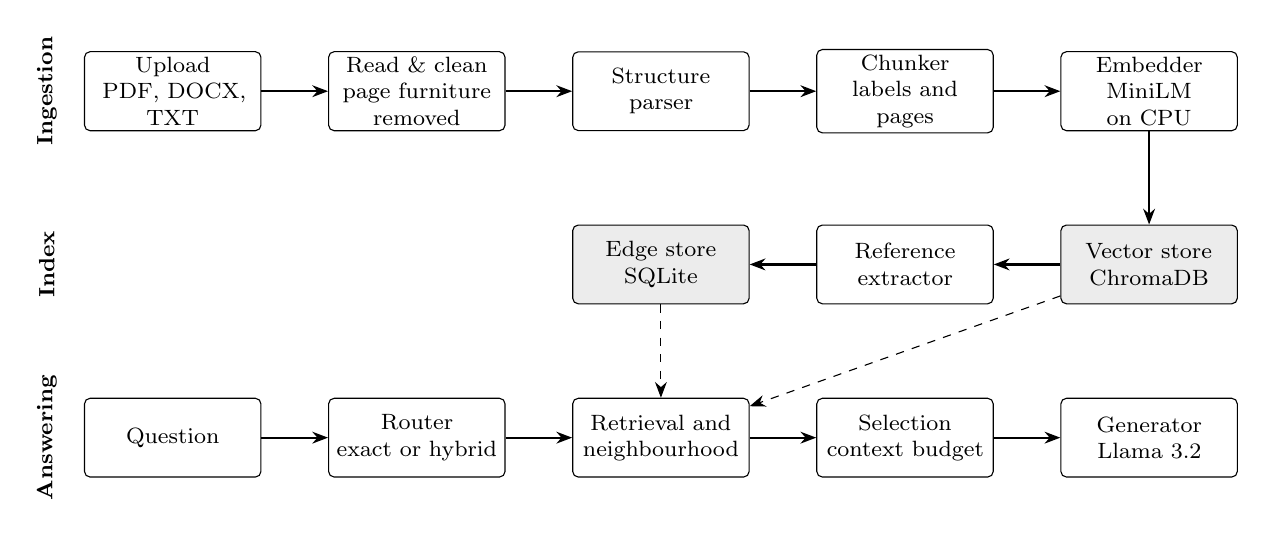
\begin{tikzpicture}[
  box/.style={draw, rounded corners=2pt, align=center, font=\footnotesize,
              text width=21mm, minimum height=10mm, inner sep=2pt},
  store/.style={box, fill=gray!15},
  flow/.style={-{Stealth[length=2mm]}, thick},
  feed/.style={-{Stealth[length=2mm]}, dashed},
  lane/.style={rotate=90, font=\footnotesize\bfseries},
]
  \node[lane] at (-1.6,0)    {Ingestion};
  \node[lane] at (-1.6,-2.2) {Index};
  \node[lane] at (-1.6,-4.4) {Answering};

  \node[box]   (upload)   at (0,0)       {Upload\\PDF, DOCX, TXT};
  \node[box]   (clean)    at (3.1,0)     {Read \& clean\\page furniture removed};
  \node[box]   (parse)    at (6.2,0)     {Structure\\parser};
  \node[box]   (chunk)    at (9.3,0)     {Chunker\\labels and pages};
  \node[box]   (embed)    at (12.4,0)    {Embedder\\MiniLM on CPU};

  \node[store] (edges)    at (6.2,-2.2)  {Edge store\\SQLite};
  \node[box]   (refs)     at (9.3,-2.2)  {Reference\\extractor};
  \node[store] (chroma)   at (12.4,-2.2) {Vector store\\ChromaDB};

  \node[box]   (question) at (0,-4.4)    {Question};
  \node[box]   (route)    at (3.1,-4.4)  {Router\\exact or hybrid};
  \node[box]   (retrieve) at (6.2,-4.4)  {Retrieval and\\neighbourhood};
  \node[box]   (select)   at (9.3,-4.4)  {Selection\\context budget};
  \node[box]   (generate) at (12.4,-4.4) {Generator\\Llama 3.2};

  \draw[flow] (upload) -- (clean);
  \draw[flow] (clean) -- (parse);
  \draw[flow] (parse) -- (chunk);
  \draw[flow] (chunk) -- (embed);
  \draw[flow] (embed) -- (chroma);
  \draw[flow] (chroma) -- (refs);
  \draw[flow] (refs) -- (edges);

  \draw[flow] (question) -- (route);
  \draw[flow] (route) -- (retrieve);
  \draw[flow] (retrieve) -- (select);
  \draw[flow] (select) -- (generate);

  \draw[feed] (chroma) -- (retrieve);
  \draw[feed] (edges) -- (retrieve);
\end{tikzpicture}
\caption{The ingestion and answering paths. Shaded nodes are persistent
stores; dashed arrows are reads from them during answering. The reference
extractor reads the stored passages back in reading order, so the edges it
produces use exactly the labels the passages carry.}
\label{fig:architecture}
\end{figure}

\begin{table}[ht]
\centering
\small
\begin{tabularx}{\textwidth}{@{}lX@{}}
\toprule
Package & Responsibility \\
\midrule
\texttt{ingestion}  & Reading PDF, DOCX and TXT files; cleaning; structural
                      parsing; chunking; printed page numbers; reference
                      extraction \\
\texttt{embedding}  & Sentence embeddings and the ChromaDB vector store,
                      including metadata lookups \\
\texttt{retrieval}  & Query parsing, routing to exact lookup, hybrid dense and
                      lexical search, passage selection \\
\texttt{generation} & The generator interface and its Ollama-backed
                      implementation \\
\texttt{graph}      & Cross-reference edges, their SQLite store and
                      neighbourhood queries \\
\texttt{pipeline}   & The two entry points, ingestion and answering; context
                      budget; deterministic replies \\
\texttt{api.py}     & FastAPI endpoints \\
\texttt{telemetry.py} & CPU, GPU and memory readings shown in the interface \\
\bottomrule
\end{tabularx}
\caption{Backend packages.}
\label{tab:packages}
\end{table}

\begin{table}[ht]
\centering
\small
\begin{tabularx}{\textwidth}{@{}llX@{}}
\toprule
Layer & Technology & Reason for the choice \\
\midrule
Pipeline        & Python 3.12              & The reference ecosystem for text
                                             processing, embeddings and model
                                             runtimes. \\
API             & FastAPI, Uvicorn         & Typed request models; the
                                             interface and the tests call the
                                             same endpoints. \\
PDF reading     & PyMuPDF, pypdf           & PyMuPDF exposes layout
                                             geometry---line positions and
                                             font sizes---which footer removal
                                             and page numbering rely on; pypdf
                                             is the fallback. \\
DOCX reading    & python-docx              & Paragraph-level access to Word
                                             documents. \\
Chunking        & LangChain text splitter  & Recursive splitting on paragraph,
                                             line, sentence and word
                                             boundaries. \\
Embeddings      & all-MiniLM-L6-v2         & 384-dimensional sentence
                                             embeddings~\cite{reimers2019sbert,wang2020minilm},
                                             fast enough on a CPU. \\
Vector store    & ChromaDB                 & Embedded and persistent; filters
                                             on metadata inside the store. \\
Lexical scoring & rank-bm25                & Okapi
                                             BM25~\cite{robertson2009bm25}
                                             without an external search
                                             engine. \\
Language model  & Llama 3.2 (3B), Ollama   & Runs locally within 4\,GB of video
                                             memory. \\
Graph store     & SQLite                   & Part of the Python standard
                                             library; no server to run. \\
Desktop shell   & Tauri 2                  & Uses the system web view, so the
                                             application stays small. \\
Interface       & React 19, TypeScript     & Typed components, built with Vite
                                             and styled with Tailwind CSS. \\
Telemetry       & psutil, NVML             & CPU, memory and GPU readings. \\
\bottomrule
\end{tabularx}
\caption{Technology stack.}
\label{tab:stack}
\end{table}

\subsection{Development timeline}

\Cref{tab:timeline} summarises how the system was built. Development
proceeded from the bottom of the pipeline upwards: ingestion first, then
retrieval and generation, then structure and cross-references, with the
interface growing alongside.

\begin{table}[ht]
\centering
\small
\begin{tabularx}{\textwidth}{@{}lX@{}}
\toprule
Period & Milestones \\
\midrule
April--May 2026      & Ingestion layer: readers for PDF, DOCX and TXT behind
                       one loader; fixed-size chunking; unit tests on a PDF
                       fixture. Local embedding layer on ChromaDB. \\
June 2026            & Generator interface and the first end-to-end pipeline,
                       retrieving by embedding similarity alone. Repository
                       split into \texttt{backend/} and \texttt{frontend/}.
                       Endpoints for health, upload and query; chat pane wired
                       to the backend; text cleaning; generation through
                       Ollama. \\
June--July 2026      & Queries scoped to one document; token usage shown per
                       answer; hybrid retrieval with BM25 and reciprocal rank
                       fusion; retrieval returns chunk identifiers and
                       metadata. \\
August 2026          & Structural markers and page boundaries kept during
                       ingestion; queries naming a provision routed to exact
                       metadata lookup; live CPU and GPU telemetry; passage
                       locations shown in the interface. \\
Early September 2026 & Passages ordered against the lost-in-the-middle
                       effect; embedder moved to the CPU; symbol-font glyphs
                       stripped; past answers replayable; per-document
                       statistics; structural units detected generically;
                       answers split into a direct answer and a supporting
                       detail. \\
Mid September 2026   & Cross-reference extraction and edge building; paragraph
                       and point labels; running headers and footers removed;
                       edges stored and a neighbourhood returned with each
                       answer; continuous integration; an interactive
                       cross-reference graph; desktop window sizing and native
                       translucency. \\
Late September 2026  & Graph view replaced by a reference tree; retrieval of
                       the exact subdivision named, with typo tolerance;
                       commands and query cancellation; printed page numbers;
                       passage count decided by the system; text that closes a
                       list recognised as a subparagraph; plain-language
                       summaries for bare references. \\
\bottomrule
\end{tabularx}
\caption{Development timeline.}
\label{tab:timeline}
\end{table}

\subsection{Structure of this report}

Part~I covers the system up to the cross-reference graph: ingestion
(\cref{sec:ingestion}), retrieval (\cref{sec:retrieval}), generation
(\cref{sec:generation}) and the interface (\cref{sec:interface}). Part~II
covers what it took to make the system output cross-references: parsing
structure below the level of a provision (\cref{sec:structure}) and the graph
built on it, including how it is presented (\cref{sec:graph}).
\Cref{sec:status} closes with the current status, measured behaviour and
limitations.


\clearpage
\part{Grounded Question Answering}
\suppressfloats[t]
\section{Ingestion}
\label{sec:ingestion}

Ingestion turns an uploaded file into passages that carry their provenance.
It runs once per upload, in the order shown in \cref{lst:ingest}: the file is
read page by page, cleaned, split into labelled chunks, given the page numbers
printed on its pages, embedded and stored, and finally scanned for
cross-references (Part~II).

\begin{lstlisting}[float, language=Python, caption={The ingestion entry point
(\texttt{pipeline/pipeline.py}).}, label={lst:ingest}]
def ingest(doc_path: str) -> int:
    pages = load_document_pages(doc_path)
    chunks = with_printed_pages(chunk_document(pages),
                                load_printed_pages(doc_path))
    doc_name = os.path.basename(doc_path)

    embed_and_store_chunks(chunks, doc_name)
    build_graph(doc_name)

    return len(chunks)
\end{lstlisting}

\subsection{Reading documents}

A single loader dispatches on the file extension to a reader for PDF, DOCX or
plain text; the interface checks the extension before uploading, and the loader
rejects any other type. The loader returns a list of (page number, text) pairs,
so that page boundaries survive into the chunks. Only PDF files have real pages;
a Word or text file is returned as a single page.

PDF files are read with PyMuPDF, which reports every line of a page together
with its bounding box and font size. This geometry matters because of two kinds
of page furniture. Footnotes and running footers sit visually below the body
text, but once the layout is flattened into a text stream they land in the
middle of it: a footnote ends up spliced into the very clause that cites it,
where it corrupts both the passage and any reference found in it. The reader
therefore walks each page's lines from the bottom up and drops the trailing run
of lines that are either smaller than the body text or lie in the bottom 5\,\%
of the page, stopping at the first line of body text. The body size is taken to
be the font size that carries the most characters on the page. A recital marker
such as ``(148)'' is also set small, but it always has body text below it, so
the walk never reaches it. If PyMuPDF fails, the reader falls back to pypdf,
which extracts text without geometry.

\subsection{Cleaning}

Extracted text is normalised before it is parsed:

\begin{itemize}
  \item Unicode is normalised to NFC, and typographic dashes, quotes, bullets
  and ellipses are mapped to plain equivalents.
  \item Box-drawing and geometric symbols are removed, together with code
  points from the Unicode Private Use Area. Symbol fonts such as Wingdings
  place their bullets there, and extraction copies them as raw code points
  that render as empty boxes.
  \item Control characters and lines consisting only of a number are removed,
  runs of spaces are collapsed, and three or more blank lines become two.
  \item Text that lost its spaces during extraction---detected when fewer
  than 8\,\% of its characters are spaces---has letter runs of twelve or more
  characters split into words with a word-frequency model (wordninja).
\end{itemize}

Running headers and footers that survive the geometric filter are removed
across pages. The first and last four lines of every page are reduced to a
\emph{signature} in which every run of digits becomes \texttt{\#}, so that
``Page 12 of 144'' and ``Page 13 of 144'' share one signature. A signature
that appears on at least $\max(3, \lfloor P/2 \rfloor)$ of the document's
$P$ pages is page furniture and is removed everywhere before the pages are
joined. The threshold is deliberately conservative: a genuine line repeated
on half of all pages is rare, whereas a running header that survives turns up
in the middle of passages and in retrieval results.

\subsection{Structural units}

Densely cross-referenced documents announce their structure in their text:
headings such as ``Article 7'', ``Chapter III'' or ``Annex VIII'', recital
numbers such as ``(148)'', and numbered paragraphs and lettered points. The
structure parser finds these markers and the chunker turns them into chunk
boundaries and labels. This section describes the units down to the level of
a provision; the subdivisions inside a provision are the subject of
\cref{sec:structure}.

A heading is a unit word---\emph{Article, Section, Clause, Rule, Annex,
Schedule, Exhibit, Appendix, Chapter, Part} or \emph{Title}---followed by a
number in any of the forms the development corpora use: \texttt{58},
\texttt{3.13}, \texttt{3.7A}, \texttt{VII} or \texttt{B}. It must stand alone
on its line or be followed by a capitalised title, which rules out sentences
that merely begin with a reference. Article numbers must also form a sequence:
the first may be at most 3, and each later one must be greater than the one
before. A heading-like line that breaks the sequence---typically a reference
to another article that happens to begin a line---is rejected. Recitals are
numbers in parentheses alone on their line and are accepted only in the order
1, 2, 3, \ldots, which rejects footnote markers of the same shape.

Each unit has a depth (\cref{tab:depths}). The parser keeps the current path
from the outermost unit to the innermost, and a marker takes over its own
depth and closes everything deeper: a new article closes the previous
article's paragraph and point, but not its chapter. Every chunk is labelled
with the full path it falls under, such as \emph{chapter} III, \emph{article}
7, \emph{paragraph} 2, \emph{point} b.

\begin{table}[ht]
\centering
\small
\begin{tabular}{@{}cl@{}}
\toprule
Depth & Units \\
\midrule
0 & annex, schedule, appendix, exhibit \\
1 & part \\
2 & title \\
3 & chapter \\
4 & section \\
5 & article, recital, clause, rule \\
6 & paragraph \\
7 & point, subparagraph \\
8 & sub-point \\
\bottomrule
\end{tabular}
\caption{Structural depths. A marker closes every open unit at its own depth
or deeper.}
\label{tab:depths}
\end{table}

None of the unit words is specific to one legal system, and none is required.
A document in which fewer than three markers are found is treated as
unstructured and chunked plainly; retrieval then relies on similarity alone.

\subsection{Chunking}

The cleaned pages are joined into one string, and the offset at which each
page starts is recorded, so that any position in the text can be mapped back
to its page by binary search. The text between two consecutive markers is
split with a recursive character splitter into chunks of at most 500
characters with an overlap of 50, preferring to break at blank lines, then
line ends, then sentence ends, then spaces. Each chunk is stored with its
text, the pages on which it starts and ends, and the structural labels of its
path.

\paragraph{Trade-offs.} Small chunks make retrieval precise: one point of a
list is usually one chunk, so a citation points at the sentence that matters
rather than at a page of text. The cost is that a long provision spans many
chunks. This is acceptable because a named provision is never retrieved by
similarity: it is reassembled from its labels in reading order
(\cref{sec:retrieval}). Cutting at markers before splitting by size also means
that no chunk straddles two provisions, so every label a chunk carries is
exact.

\subsection{Printed page numbers}

The page number a reader sees is often not the PDF's own page index. Front
matter pushes the printed numbering behind: the page of TCPS~2 that prints
``48'' is the 56th page of the PDF. A reader who asks about ``page 48'' means
the printed number, and a citation should show it. The printed number sits in
the footer, which the reader has just removed, so it is recovered from the
page geometry instead.

For every page $p$, the numbers standing at the start or end of a line in the
top and bottom 8\,\% of the page are collected, including the first number of
forms such as ``117/144'' and ``L~176/5''. Each such number $n$ proposes an
offset $p - n$. Let $G_p$ be the set of offsets proposed on page $p$. The
document's offset is the one proposed by the most pages,
\begin{equation}
  o^{*} = \arg\max_{o} \bigl|\{\, p : o \in G_p \,\}\bigr|,
\end{equation}
and it is accepted only if at least $\max(3, P/2)$ of the $P$ pages agree on
it. Every page $p$ with $p - o^{*} \geq 1$ is then given the printed number
$p - o^{*}$, and every chunk receives the printed numbers of the pages on
which it starts and ends. For TCPS~2 the offset is 8; for the AI Act, whose
footers read ``117/144'', it is 0.

The agreement threshold is what keeps this general. Numbers in the margins
that are not page numbers---dates, article numbers, journal
references---propose offsets that vary from page to page and never
accumulate. A document
numbered per section (``3.8-2'') or not at all never reaches agreement and
keeps the PDF numbering, which is the correct fallback. The method assumes a
single dominant numbering run: front matter numbered in roman numerals simply
receives no printed number, and a document whose numbering restarts several
times is numbered by its longest run.

\subsection{Embedding and storage}

Chunks are embedded with all-MiniLM-L6-v2~\cite{wang2020minilm}, a
sentence-transformer~\cite{reimers2019sbert} that maps text to a
384-dimensional vector, and stored in a persistent ChromaDB collection that
uses cosine distance. Each chunk's identifier is
\texttt{\{document\}\_chunk\_\{i\}}, so reading order can be recovered by
sorting identifiers. Its metadata holds the source document, the start and end
pages (PDF and printed) and the structural labels. Plain numbers are stored as
integers and all other identifiers as text (\texttt{58} but \texttt{"3.7A"}),
because the store's equality filters are typed. Uploading a document again
first deletes its previous chunks, and writes are batched below the store's
maximum batch size, which large regulations exceed.

\paragraph{Trade-offs.} The embedder runs on the CPU. On a 4\,GB GPU every
megabyte of video memory taken by the embedder is a megabyte the language
model cannot use, and the model already has to offload part of its layers to
system memory. Embedding a large document on the CPU takes longer, but it
happens once per upload, and a query needs only one short text embedded.
ChromaDB was chosen over a bare vector index such as FAISS because it
evaluates metadata filters---equality, conjunction, disjunction and numeric
ranges---inside the store, which exact lookups (\cref{sec:retrieval}) depend
on. Its filters offer no substring or pattern matching, which is why the
parsing effort goes into producing exact labels at ingestion rather than into
matching loosely at query time.

\section{Retrieval}
\label{sec:retrieval}

Retrieval decides which passages the language model sees, and therefore bounds
what any answer can say. It has two paths. A question that names a location in
a document is answered by \emph{exact lookup} on the stored labels; any other
question goes to \emph{hybrid search}, which combines semantic and lexical
similarity. The router tries exact lookup first and falls back to hybrid search
when the question names nothing or nothing carries the named labels. Besides
the passages, it returns a note stating whether the lookup was exact, which
subdivision the question asked for, whether that subdivision was found, and,
if not, what the provision contains instead (\cref{sec:structure}).

\subsection{Hybrid search}

\paragraph{Dense ranking.} The question is embedded with the same model as the
passages, and every chunk in scope---one selected document or the whole
collection---is ranked by cosine distance to it.

\paragraph{Lexical ranking.} The same chunks are ranked by Okapi
BM25~\cite{robertson2009bm25} over lower-cased word tokens.

\paragraph{Fusion.} The two rankings are combined by reciprocal rank
fusion~\cite{cormack2009rrf} (\cref{lst:rrf}). Each chunk $d$ scores
\begin{equation}
  \operatorname{RRF}(d) = \sum_{r \in \{\mathrm{dense},\, \mathrm{BM25}\}}
  \frac{1}{k + \operatorname{rank}_r(d)}, \qquad k = 60,
\end{equation}
where $\operatorname{rank}_r(d)$ is the chunk's position in ranking $r$,
counted from 0.

\begin{lstlisting}[float, language=Python, caption={Reciprocal rank fusion
(\texttt{retrieval/hybrid.py}).}, label={lst:rrf}]
def _rrf(rank_list: list[list[str]], k: int = 60) -> dict:
    scores: dict[str, float] = {}
    for ranking in rank_list:
        for rank, _id in enumerate(ranking):
            scores[_id] = scores.get(_id, 0.0) + 1.0 / (k + rank)
    return scores
\end{lstlisting}

\paragraph{Trade-offs.} The two rankings fail in complementary ways. Dense
embeddings capture paraphrase---``who can complain'' finds a provision on the
right to lodge a complaint---but blur exact tokens: numbers, amounts and
defined terms (``Article~92'', ``EUR~15\,000\,000'') contribute little to a
sentence vector. BM25 matches exact tokens but knows nothing of synonyms.
Fusing by rank rather than by score avoids having to reconcile two
incomparable scales, a bounded cosine distance and an unbounded BM25 score,
and needs no tuned weights. The cost is that magnitudes are discarded: a
passage far ahead in one ranking gets no more credit than one narrowly ahead.
The BM25 index is rebuilt over the chunks in scope for each question. Over the
2\,019 chunks of the AI Act, hybrid retrieval takes about 235\,ms in total,
which is small beside generation; a collection orders of magnitude larger
would need a persistent inverted index instead.

\subsection{Exact lookup for named locations}

\paragraph{Parsing the question.} A pattern finds unit words followed by a
number (``article 66'', ``Art.~66'', ``articles no.~5'', ``page 48'',
``section 3.13''). Plain numbers become integers and anything else upper-cased
text, matching how the labels were stored (\texttt{3.7a} matches
\texttt{3.7A}). Some conventions name a unit by another word, so a unit is
also tried under an alternative reading: in EU acts, ``clause 148'' means
recital 148, and ``section 5'' may mean article 5. A question that matches
nothing is checked for a mistyped unit word: any word of four to ten letters
followed by a number is compared with the unit vocabulary, and a similarity
ratio of at least 0.75 accepts it, so ``artilce 66'' is read as article 66.

\paragraph{Building filters.} Each named unit becomes one or more filters on
the stored metadata. A page becomes a range condition, because a chunk may run
over two pages: first on the printed page numbers, then on the PDF's own page
numbers (\cref{lst:page}). When a question names several units, all of them
are combined first, so that ``chapter 3 page 48'' retrieves the passages on
printed page 48 \emph{within} chapter 3. Only if no chunk carries them all is
each unit tried on its own, the most specific first: page, then recital,
clause, rule, article, section, annex, schedule, chapter and part. Trying the
units separately from the outset returns chapter 3's opening passages for that
question, because ``chapter 3'' alone matches first; the combination is what
lets a page be addressed inside a chapter.

\begin{lstlisting}[float, language=Python, caption={Filters for one named unit; a
page matches every chunk that runs over it (\texttt{retrieval/hybrid.py}).},
label={lst:page}]
def _alternatives(field, value):
    if field != "page":
        return [{field: {"$eq": value}}]
    if not isinstance(value, int):
        return []

    return [
        {"$and": [{"printed_page": {"$lte": value}},
                  {"printed_page_end": {"$gte": value}}]},
        {"$and": [{"page": {"$lte": value}},
                  {"page_end": {"$gte": value}}]},
        {"page": {"$eq": value}},
    ]
\end{lstlisting}

\paragraph{Returning the provision.} The first filter that matches returns
every chunk of the provision, up to 200, in reading order---not the
$k$ most similar chunks. A named provision is the answer to ``what does it
say'' in full, and similarity has no role in deciding which of its parts
matter. The subdivisions inside it are handled in \cref{sec:structure}.

\paragraph{Trade-offs.} Exact lookup is deterministic and explainable: the
same question always returns the same passages, and the interface can say
``exact match'' instead of presenting a similarity score as if it measured
correctness. It is also fast, taking 3--6\,ms against roughly 235\,ms for
hybrid search. Its weakness is that it depends on the question naming units in
a form the parser recognises. A form it does not recognise falls through to
hybrid search, so the worst case is the behaviour of an ordinary RAG system,
never an empty answer.

\subsection{Deciding how many passages}

Early versions let the user choose how many passages to retrieve, between 2
and 12. A fixed number fits no question well: it truncates a long provision
that was named in full, and it pads a focused question with passages that
merely share its vocabulary. The number is now decided by the system, from
what the question asked for:

\begin{itemize}
  \item \textbf{A named subdivision} (``paragraph 2 of Article 7''): exactly
  the chunks that carry the requested labels, which for a paragraph includes
  all of its points and sub-points (\cref{sec:structure}).
  \item \textbf{A named provision} (``Article 93''): the whole provision in
  reading order.
  \item \textbf{Any other question}: the candidates that score close to the
  best one. Of the twelve best candidates after fusion, candidate $i$
  (counted from 0) is kept if
  \begin{equation}
    i < 3 \quad\text{or}\quad s_i \geq \max_j s_j - 0.15,
  \end{equation}
  where $s_i$ is its cosine similarity to the question, and at most eight are
  kept (\cref{lst:close}).
\end{itemize}

On every path the passages are then admitted in order while their total length
stays within 2\,000 words. At about 1.4 tokens per word this is roughly 2\,800
tokens, which leaves room in the model's 4\,096-token context window for the
instructions and the answer.

\begin{lstlisting}[float, language=Python, caption={Keeping the passages close to the
best one (\texttt{retrieval/hybrid.py}).}, label={lst:close}]
def _close_to_best(chunks, distances, metas):
    if not distances:
        return chunks, distances, metas

    best = 1 - min(distances)
    keep = []
    for i, distance in enumerate(distances):
        if i < _FEWEST or 1 - distance >= best - _MARGIN:
            keep.append(i)
    keep = keep[:_MOST]

    return ([chunks[i] for i in keep], [distances[i] for i in keep],
            [metas[i] for i in keep])
\end{lstlisting}

\paragraph{Trade-offs.} The margin is relative rather than absolute because
similarities between a question and the passages of one document cluster
tightly: for typical questions on the AI Act the top twelve candidates fell
between 0.57 and 0.86, so an absolute threshold would keep everything for one
question and nothing for the next. The minimum of three protects against a
lone passage cut mid-sentence, and the maximum of eight against a question so
generic that everything scores alike. The margin and bounds were set by
inspecting score distributions on the development corpora rather than learned,
and they fix only the upper limit; the context budget decides the rest.

\section{Generation}
\label{sec:generation}

\subsection{Model and runtime}

Answers are generated by Llama~3.2 with 3 billion parameters, served locally by
Ollama with a 4\,096-token context window, a temperature of 0 and JSON output
mode. At temperature 0 the same passages and question produce the same answer,
which makes behaviour reproducible and differences between versions of the
pipeline attributable to the pipeline. On the development machine about four
fifths of the model's layers fit in the 4\,GB of video memory and the rest run
from system memory, so generation speed is bounded by memory bandwidth rather
than by the GPU: an answer takes 7--9\,s once the model is loaded, and about
20\,s when it has to be loaded first. The interface warns in advance when the
model is not loaded.

The generator sits behind an abstract interface with a single method,
\texttt{generate(query, chunks, focus)}, so a different model or runtime can
be substituted by adding one class without touching retrieval or the API.

\paragraph{Trade-offs.} A local 3B model keeps every document on the machine,
costs nothing per question and works offline. The price is weaker synthesis
than a large hosted model and a small context window. Both push work into
retrieval: the passages must already be the right ones, in the right order,
and within budget, because the model cannot compensate for a poor selection.

\subsection{Prompt}

The prompt (\cref{lst:prompt}) states the model's role, gives it two tasks,
tells it what to do when the passages do not contain the answer, and fixes the
shape of its output. The \emph{answer} responds to the question directly; the
\emph{detail} states where in the document the answer comes from, citing
passages by number, and says plainly when the document only names something
without describing it.

\begin{lstlisting}[float, caption={The prompt, abridged
(\texttt{generation/basic\_backend.py}).}, label={lst:prompt}]
[The question names Article 101(1). The passages below are that
text; answer from them.]
You answer questions about a document using ONLY the numbered
context passages below.
Do two things:
1. ANSWER: answer the question directly and briefly.
2. DETAIL: say where in the document the answer comes from and what
   the surrounding text adds, citing passages by their number,
   e.g. [2]. If the document only names something without
   describing it, say so plainly instead of repeating the name.
Do not add anything the passages do not say.
If the passages do not contain the answer, say that they do not.
Respond with a JSON object EXACTLY in this shape:
{ "answer": "...", "detail": "..." }

Context:
[1] ...
[3] ...
[2] ...

Question: ...
\end{lstlisting}

\paragraph{Passage order.} Language models attend most reliably to the start
and end of a long context and least to its middle~\cite{liu2024lost}. The
passages arrive ranked, so they are interleaved before being placed in the
prompt: the first, third, fifth and so on from the front, then the rest in
reverse, which puts the strongest passages at both ends (for six passages the
order is 1, 3, 5, 6, 4, 2). Each passage keeps the number it had before
reordering, and that number is the one the interface shows, so ``[3]'' in the
detail is Source~3 in the citations pane.

\paragraph{Focus.} When exact lookup found the subdivision the question named,
the prompt opens with a line naming it: ``The question names Article 101(1).
The passages below are that text; answer from them.'' Without it, a small
model treats the passages as loose matches and may answer from a neighbouring
passage that reads as relevant.

\subsection{Deterministic replies}

Three situations are answered without relying on the model's judgement.

\paragraph{A named part that does not exist.} A question may name a
subdivision the provision does not have, such as paragraph 2 of an article
that is a single paragraph. Given the rest of the article, a small model
answers anyway, presenting a neighbouring sentence as the requested paragraph.
The model is therefore not called. The reply is composed from the stored
labels, and the whole provision is shown in the citations pane:

\begin{quote}\small
Article 85 has no paragraph 2: its text is not divided into paragraphs.\\
Article 7 has no paragraph 9. Its paragraphs are 1, 2, 3.
\end{quote}

\paragraph{A bare reference.} A query such as ``paragraph 1 article 101''
names a location but asks nothing, and with nothing to answer the model tends
to return an empty answer. A query is treated as a bare reference when nothing
but filler words (``show'', ``the text of'') remains once every recognised
reference is removed from it. The question given to the model is then replaced
by a task that makes the chat reply worth having next to the passages
themselves: ``Explain in plain language what Article 101(1) says.''

\paragraph{A non-answer.} If the model's answer is empty or a placeholder
(``None'', ``null'', ``N/A'', ``unknown''), it is replaced by a notice that
the passages are in the citations pane, rather than displayed as if it were
an answer.

\subsection{Response}

Every answer is returned as one JSON object: the answer and its detail; the
passages; for each passage, its document, pages and structural labels; the
cross-reference neighbourhood of the passages (\cref{sec:graph}); the lookup
note; retrieval and generation times; and the prompt and completion token
counts reported by Ollama together with the size of the context window.

\paragraph{No relevance percentage.} Earlier versions showed a relevance
percentage for each passage, derived from its cosine similarity to the
question. It was removed because it measured how closely the wording matched,
not whether the answer was right, and because passages found by exact lookup
always showed 100\,\%. The lookup note replaced it: the interface states
whether the passages are an exact match on the named provision or the closest
passages by keyword and meaning, which is what the reader needs in order to
judge them.

\section{Interface}
\label{sec:interface}

\subsection{HTTP API}

The backend is served by FastAPI (\cref{tab:api}). Answering and retrieval
take the same request, a query and an optional document to scope it to. The
number of passages is deliberately not a parameter: it is decided by the
retrieval (\cref{sec:retrieval}).

\begin{table}[ht]
\centering
\small
\begin{tabularx}{\textwidth}{@{}llX@{}}
\toprule
Method & Path & Purpose \\
\midrule
GET    & \texttt{/health}                     & Liveness check. \\
GET    & \texttt{/stats}                      & CPU, GPU and memory load and
                                                temperatures. \\
GET    & \texttt{/documents}                  & Indexed documents and their
                                                chunk counts. \\
POST   & \texttt{/upload}                     & Store and ingest a file. \\
DELETE & \texttt{/document/\{name\}}          & Remove a document's chunks and
                                                cross-reference edges. \\
GET    & \texttt{/document/\{name\}/stats}    & Pages and structural units
                                                found. \\
POST   & \texttt{/query}                      & Retrieval-augmented answer. \\
POST   & \texttt{/retrieve}                   & Passages only, without
                                                generation. \\
GET    & \texttt{/document/\{name\}/provision}  & Full text of one provision,
                                                in reading order. \\
GET    & \texttt{/document/\{name\}/neighbours} & What a provision cites and
                                                what cites it. \\
\bottomrule
\end{tabularx}
\caption{API endpoints.}
\label{tab:api}
\end{table}

\subsection{Desktop application}

The interface is a React~19 application written in TypeScript and built with
Vite, running inside a Tauri~2 desktop shell. It is divided into three
resizable panes that can each be folded away (\cref{fig:interface}).

\begin{figure}[ht]
\centering
\IfFileExists{images/interface.png}{%
  \includegraphics[width=\textwidth]{images/interface.png}%
}{%
  \fbox{\parbox{0.9\textwidth}{\centering\small
  Screenshot of the application: save it as \texttt{images/interface.png}.}}%
}
\caption{The desktop application: retrieved citations (left), chat (centre)
and context (right).}
\label{fig:interface}
\end{figure}

\paragraph{Retrieved citations.} Each passage is shown as a card headed by its
source number, its printed page and its reference written the way it would be
cited---for example ``p.~118 $\cdot$ Article 101(1), second subparagraph''. A
line above the cards states how the passages were found: an exact match on the
provision named, or the closest passages by keyword and meaning. Below each
card, the provisions the passage cites can be followed (\cref{sec:graph}).

\paragraph{Chat.} The transcript shows the question, the answer, and the
detail beneath it in smaller type. Every answered turn keeps its own passages,
so clicking an earlier answer restores its citations without querying again. A
running query can be stopped. The composer shows which document questions are
scoped to and accepts a small set of commands, suggested as the first word is
typed: \texttt{find:} retrieves passages without generating an answer,
\texttt{doc:} changes the scope, \texttt{clear} empties the conversation and
\texttt{help} lists the commands. Shorthand for structural words is expanded
with the Tab key: \texttt{a}, \texttt{para}, \texttt{p}, \texttt{sec} and
\texttt{cha} become \emph{article}, \emph{paragraph}, \emph{point},
\emph{section} and \emph{chapter}. Only Tab expands, so the word ``a'' in an
ordinary sentence is left alone.

\paragraph{Context.} The last query's token usage is shown against the
4\,096-token window, split into prompt and response, together with the
session total and the time taken. Machine telemetry shows GPU and CPU load,
temperature and memory, and how much of the model is resident in video
memory. The document list shows each indexed document with a structural
summary (``144 pages $\cdot$ 13 chapters $\cdot$ 113 articles $\cdot$ 180
recitals''), accepts uploads of PDF, DOCX and TXT files with an estimate of
the indexing time, and scopes questions to a document when it is clicked.

\paragraph{Trade-offs.} Tauri was chosen over Electron because it uses the
operating system's web view instead of bundling a browser, which keeps the
application small and its memory footprint low beside a language model
competing for the same machine. The cost is that three web engines render the
interface---WebKit on macOS and Linux, WebView2 on Windows---and small
differences between them must be accommodated. Native translucency is used
only where the platform composites it itself (vibrancy on macOS, Mica and
Acrylic on Windows); elsewhere the window stays opaque, because a blur
redrawn by the web view on every change of the panes made the interface
sluggish.


\clearpage
\part{Cross-Referencing}
\suppressfloats[t]
\section{Structure below the provision}
\label{sec:structure}

Cross-references in dense documents rarely point at a whole provision. They
point inside one: ``Article 66(2)(e)(iv)'', ``paragraph 1, point (b)'', ``the
second subparagraph of paragraph 3''. Readers ask questions the same way. To
resolve either, every passage has to know not only its article but its
paragraph, point, sub-point and subparagraph. This was the first thing it took
to make the system output cross-references: until passages carry these labels,
a reference can be resolved only to a whole provision, and ``Article 66(2)(e)''
cannot be told apart from Article 66.

\subsection{Paragraphs, points and sub-points}

Inside a provision three kinds of marker open a line: a numbered paragraph
(``2.''), a lettered point (``(b)'' or ``b.'') and a roman sub-point (``(iv)''
or ``iv.''). The shapes alone are ambiguous: ``(i)'', ``(v)'' and ``(x)'' are
both letters and roman numerals, and a number followed by a full stop can begin
a wrapped line in the middle of a sentence.

The parser therefore resolves markers by \emph{sequence}. After each heading it
expects paragraph 1 and point (a); it then tracks the next paragraph number,
the next point letter and, once a point is open, the next roman numeral. A
marker is accepted only if it is the one expected next (\cref{lst:sequence}).
After point (h), ``(i)'' is the expected letter and becomes point (i). After
point (k) of Article 7(2) of the AI Act---``the extent to which existing Union
law provides for:''---the expected letter is (l), so the ``(i)'' that follows
is taken as the first sub-point of (k). A paragraph number is accepted only if
it is the next one expected and the text before it ends a sentence or a clause
(with ``.'', ``;'' or ``:''), which rejects numbers that merely begin a line.

\begin{lstlisting}[float, language=Python, caption={Accepting a point or sub-point
only in sequence (\texttt{ingestion/structure.py}, abridged).},
label={lst:sequence}]
elif kind == "marker" and next_paragraph is not None:
    if value == next_point:
        marks.append((pos, "point", value))
        next_point = chr(ord(value) + 1)
        next_subpoint = "i"
    elif value == next_subpoint:
        marks.append((pos, "subpoint", value))
        index = _ROMANS.index(value)
        if index + 1 < len(_ROMANS):
            next_subpoint = _ROMANS[index + 1]
        else:
            next_subpoint = None
\end{lstlisting}

\subsection{Text that closes a list}

A paragraph that introduces a list of points often continues after the list
with text that applies to the whole paragraph, not to its last point. EU
drafting calls it a \emph{subparagraph}. Article 101(1) of the AI Act lists
four grounds for a fine in points (a) to (d) and then states, without a marker
of its own, how the amount of the fine is fixed. Nothing in the text marks
where point (d) ends, so a parser that only reads markers would give the
fining criteria the label of point (d)---and a question about point (d) would
receive them too.

The end of a list is recognised from the punctuation of formal drafting. Items
before the last end with a semicolon, a comma or a conjunction; only the last
ends a sentence. So after the last item of a list, a full stop followed by a
line that begins with a capital letter starts the closing text. Inside a
numbered paragraph the closing text is labelled as the paragraph's second
subparagraph (third, and so on, after further lists); outside a numbered
paragraph there is no subparagraph to name, and the closing text simply
returns to the level of the provision. This also covers documents other than
legislation: without it, the guidance that follows the conditions listed in
TCPS~2 Article 3.7A would carry the label of its last condition.
\Cref{lst:article101} shows the labels the chunks of Article 101 receive.

\begin{lstlisting}[float, numbers=none, caption={Labels assigned to the chunks of
Article 101 of the AI Act.}, label={lst:article101}]
p.117  Article 101               Article 101 Fines for providers of ...
p.117  Article 101(1)            1. The Commission may impose ... fines
p.117  Article 101(1)(a)         (a) infringed the relevant provisions ...
p.117  Article 101(1)(b)         (b) failed to comply with a request ...
p.117  Article 101(1)(c)         (c) failed to comply with a measure ...
p.118  Article 101(1)(d)         (d) failed to make available ...
p.118  Article 101(1), 2nd sub.  In fixing the amount of the fine ...
p.118  Article 101(2)            2. Before adopting the decision ...
\end{lstlisting}

\paragraph{Trade-offs.} The rule relies on drafting conventions rather than
on layout, so it works on text extracted from any source. It would close a
list too early if its last item ran over several sentences with a line break
after the first, which formal drafting rarely does. Articles whose lists are
not followed by closing text, such as Article 7 of the AI Act, are labelled
exactly as before.

\subsection{Asking for a subdivision}

The question is parsed for the subdivision it names (\cref{tab:subdivisions}).
A single letter is a point and two or more roman letters are a sub-point, so
``point (i)'' reads as a point and ``point (iv)'' as a sub-point. A number
after \emph{point} or \emph{item} is read as a paragraph, because that is how
people refer to numbered paragraphs in practice.

\begin{table}[ht]
\centering
\small
\begin{tabular}{@{}ll@{}}
\toprule
Written in the question & Read as \\
\midrule
paragraph 2, para 2, subsection 2, 66(2)  & paragraph 2 \\
point d, letter d, (d)                    & point d \\
point (iv), subpoint iv, (iv)             & sub-point iv \\
point 3, item 3                           & paragraph 3 \\
second subparagraph, subparagraph 2       & subparagraph 2 \\
\bottomrule
\end{tabular}
\caption{Subdivisions recognised in a question.}
\label{tab:subdivisions}
\end{table}

Exact lookup (\cref{sec:retrieval}) fetches the whole provision, and the
chunks that carry every requested label are then kept; a paragraph's first
subparagraph is its text without a subparagraph label. If no chunk carries
them all, the outer labels are dropped one at a time, so ``66(2)(e)'' still
finds point (e) in an article whose points are not grouped into numbered
paragraphs. Only the matching chunks are passed on: ``paragraph 2 of Article
7'' returns 14 chunks---the paragraph's opening, points (a) to (k), and the two
sub-points of point (k)---while ``point (k) of paragraph 2 of Article 7''
returns three, and ``the second subparagraph of paragraph 1 of Article 101''
returns the closing text alone. When the provision has no such subdivision, the
lookup note lists what it has instead, which produces the deterministic reply
described in \cref{sec:generation}.

\subsection{Writing references for the reader}

A passage's labels are written back the way the reference would be cited:
the provision, then the paragraph, point and sub-point in parentheses, then the
subparagraph in words---``Article 66(2)(e)(iv)'', ``Article 101(1), second
subparagraph''---preceded by the printed page where the document has one. The
same wording is used for the focus line given to the model
(\cref{sec:generation}), so the model and the reader see the same reference.

\section{Cross-reference graph}
\label{sec:graph}

With passages labelled down to their subdivisions, the references between them
can be resolved. The graph is built once per upload, stored beside the vectors,
and read at answer time. This section follows it through its five stages:
extracting references, turning them into edges, storing them, expanding the
neighbourhood of an answer, and presenting it to the reader.

\subsection{Extracting references}

A reference is a unit word followed by an identifier and, optionally, a
paragraph in parentheses, as in ``Article 5(2)''. The extractor uses the same
unit vocabulary as the structure parser, so anything that can be cited can
also be a heading, and the reverse. A match that stands alone on its line is a
heading, not a reference, and is skipped.

Each reference is then classified as internal or external. It points at
another instrument when it is followed by ``of'' and a capitalised name that
is not itself a unit (``Article 11 of Regulation (EU) 2019/2144''), or by an
acronym of three or more capitals (``Article 114 TFEU''). ``Article 5 of this
Regulation'' stays internal, because ``this'' is not a name. References are
deduplicated per passage by unit, identifier and instrument.
\Cref{lst:references} shows the result on a sample passage.

\begin{lstlisting}[float, numbers=none, caption={References extracted from a sample
passage.}, label={lst:references}]
1. As referred to in Article 5(2) and Annex III, the requirements of
Chapter III, Section 2 apply. Article 11 of Regulation (EU) 2019/2144
applies, as does Article 114 TFEU. See also Article 5 of this Regulation.

article 5, paragraph 2    internal
annex III                 internal
chapter III               internal
section 2                 internal
article 11                external: Regulation (EU) 2019/2144
article 114               external: TFEU
\end{lstlisting}

\subsection{Building edges}

A node is a provision: the most specific provision-level label a passage
carries---recital, article, clause, rule, section, annex, schedule, appendix,
exhibit, chapter, part or title---written as \texttt{kind:value}, for example
\texttt{article:66}. The builder reads the document's passages back from the
vector store in reading order and, for each reference in each passage, adds an
edge from the passage's provision to the provision cited. An edge is
\emph{internal} when some passage of the document carries the cited label,
\emph{external} when it names another instrument, and \emph{unresolved} when
the document has no passage with that label. A provision's references to
itself are skipped. Every edge also records its \emph{position}, the index of
the citing passage, which orders a provision's references as they appear in
the text, and its \emph{locator}, the paragraph, subparagraph, point and
sub-point of the citing passage (``paragraph 1 $\cdot$ point b'').

Reading the passages back from the store, rather than from the parser's
output, guarantees that edges use exactly the labels retrieval uses: a node
identifier converts directly into the metadata filter that fetches its text.

\paragraph{Trade-offs.} Nodes are provisions, not paragraphs. References to
``Article 5(2)'' and ``Article 5(3)'' therefore reach the same node, and the
precision on the cited side is traded for a graph that stays small and whose
every node can be fetched with one filter. Precision on the citing side is
kept in the locator. For the AI Act the graph holds 575 internal edges, 79
edges to other instruments and 29 unresolved ones, the latter mostly
references to units the parser does not label as provisions, such as the
sections inside an annex.

\subsection{Storage}

Edges are stored in SQLite (\cref{lst:schema}). A document's edges are
replaced whenever it is uploaded and removed when it is deleted. Two queries
serve every use: the edges leaving a set of nodes, ordered by position, and
the edges arriving at a set of nodes, which the index on the target makes
cheap.

\begin{lstlisting}[float, language=SQL, caption={The edge table
(\texttt{graph/store.py}).}, label={lst:schema}]
CREATE TABLE IF NOT EXISTS edges (
    position    INTEGER NOT NULL,
    locator     TEXT NOT NULL,
    document    TEXT NOT NULL,
    source      TEXT NOT NULL,
    target      TEXT NOT NULL,
    edge_type   TEXT NOT NULL,
    PRIMARY KEY (document, source, target, position)
);
CREATE INDEX IF NOT EXISTS edges_by_target ON edges (document, target);
\end{lstlisting}

\paragraph{Trade-offs.} A graph database would add a server to install and
run, for queries that are all one hop long. SQLite ships with Python, keeps
the edges in a single file beside the vector store, and answers both queries
from an index. Traversals longer than one hop are done in Python with a
bounded depth, which is all the interface needs.

\subsection{Neighbourhood of an answer}

Every answer carries the cross-reference neighbourhood of its passages. The
provisions of the retrieved passages are the seeds, at depth 0. The
neighbourhood is then expanded breadth-first along internal edges to depth 2,
with at most 50 nodes. Each node carries its label, its kind (retrieved,
internal, external or unresolved), its depth and, for provisions in the
document, a preview of its first 240 characters. Each edge carries its type,
its locator and an index that numbers a provision's references in reading
order. Because the first level arrives with the answer, the references of a
retrieved passage can be listed without another request.

Two endpoints serve deeper exploration on demand: one returns what a
provision cites and what cites it, each in reading order, and the other
returns a provision's full text (\cref{tab:api}).

\subsection{Presenting cross-references}

\paragraph{A graph view, and why it was dropped.} The first presentation was
an interactive graph drawn beside the answer, first with a force-directed
layout and then with a radial one that placed the retrieved provisions at the
centre, arranged each further level on a wider ring, swapped nodes to shorten
and uncross the arrows, and routed curved arrows around the boxes. It took
about 1\,500 lines of TypeScript. With the typical neighbourhood of 20 to 50
nodes it showed \emph{that} provisions referred to each other, but not
\emph{what} they said: reading a chain meant opening node after node while
holding the path in memory, and the layout's motion competed with the text.
The graph view was therefore dropped in favour of a much simpler interface,
and the graph itself remained in the backend as the data behind it.

\paragraph{The reference tree.} Under each citation card, the provisions the
passage cites are listed in the order the text cites them, each with the
locator of the citing passage (\cref{lst:tree}). Opening a row fetches the
cited provision's text and its own references once and shows them indented
beneath it, so a chain of citations stays on screen and reads from top to
bottom. A reference to another instrument is marked \emph{other document}, an
unresolved one \emph{not found}, and a provision that already appears higher
on the same path \emph{already above}; none of these can be opened, which also
makes every chain finite even when provisions cite each other. A long list
shows twelve rows and offers the rest on request. Nothing animates, and every
row exposes its open or closed state to assistive technology.

\begin{lstlisting}[float, numbers=none, caption={The reference tree under Article
101(1), with two levels opened (\texttt{v} open, \texttt{>} closed).},
label={lst:tree}]
Cites
v 1. Article 91 . paragraph 1 . point b
     Article 91 Power to request documentation and information
     1. The Commission may request the provider of the general-purpose
        AI model concerned to provide the documentation ...
     v 1. Article 68 . paragraph 3
          Article 68 Scientific panel of independent experts
          1. The Commission shall, by means of an implementing act, ...
> 2. Article 93 . paragraph 1 . point c
\end{lstlisting}

\paragraph{Trade-offs.} The tree gives up the overview of the whole
neighbourhood that a graph offers at a glance, and with it the ability to see
clusters and hubs. In exchange, the text of every cited provision is readable
in place and in order, which is what following a cross-reference is for. The
component is about 140 lines, a tenth of the graph view, and costs two small
requests per opened row instead of a layout computation on every change.


\part*{Status and Outlook}
\addcontentsline{toc}{part}{Status and Outlook}
\suppressfloats[t]
\section{Status and limitations}
\label{sec:status}

\subsection{Testing and continuous integration}

The unit tests run without a language model. The ingestion tests check the
PDF, Word and text readers and the chunk sizes. The generation tests replace
Ollama with a stub that records the prompt, and check that the answer and
detail are taken from the model's JSON reply, that a reply which is not JSON
is kept as the answer, that token usage is reported, that the focus line
appears exactly when a named provision was found, and that interleaving keeps
the strongest passage first. A pipeline test ingests a PDF fixture and checks
that retrieval returns passages with their locations; it needs the embedding
model and the vector store and is run locally.

Continuous integration runs on GitHub Actions for every pull request and every
push to the main branch. One job installs the interface's dependencies,
type-checks it and builds it; the other installs the backend on Python 3.12
with a CPU-only build of PyTorch and runs the eleven model-free tests.

\subsection{Measured behaviour}

\Cref{tab:corpora} lists what ingestion recovers from the two main development
documents, and \cref{tab:measured} how representative questions are served.
Times were measured on the development machine described in
\cref{sec:overview}.

\begin{table}[ht]
\centering
\small
\begin{tabularx}{\textwidth}{@{}lrrX@{}}
\toprule
Document & Pages & Chunks & Structure found \\
\midrule
AI Act~\cite{euaiact} & 144 & 2\,019 & 13 chapters, 5 sections, 113 articles,
                                       180 recitals, 13 annexes; printed pages
                                       equal PDF pages \\
TCPS~2 (2022)~\cite{tcps2} & 287 & 1\,664 & 13 chapters, 142 articles; printed
                                       page = PDF page $-$ 8 \\
\bottomrule
\end{tabularx}
\caption{Structure recovered at ingestion.}
\label{tab:corpora}
\end{table}

\begin{table}[ht]
\centering
\small
\begin{tabularx}{\textwidth}{@{}Xlrr@{}}
\toprule
Question & Path & Passages & Retrieval \\
\midrule
``paragraph 2 article 7'' (AI Act) & exact, subdivision & 14 & 3.1\,ms \\
``chapter 3 page 48'' (TCPS~2) & exact, chapter and page & 7 & 5.5\,ms \\
``paragraph 2 article 85'' (AI Act) & exact, part missing & 2 & -- \\
``who can lodge a complaint with a market surveillance authority'' (AI Act)
  & hybrid & 5 & 235\,ms \\
\bottomrule
\end{tabularx}
\caption{Retrieval for representative questions. For the missing paragraph
the reply is composed without calling the model; for the hybrid question the
provision on the right to lodge a complaint, Article 85, is ranked first.
Generating an answer adds 7--9\,s once the model is loaded.}
\label{tab:measured}
\end{table}

\subsection{Limitations}

\begin{itemize}
  \item Structure is recognised from the numbering and punctuation
  conventions of formal drafting. A document that does not follow them is
  chunked without labels and searched by similarity only.
  \item A question is resolved to one provision at a time. A question relating
  two provisions (``what does paragraph 3 of this article have to do with
  Article 7'') retrieves only one of them.
  \item References to other instruments are recognised and marked, but not
  followed into other uploaded documents.
  \item The local 3B model and its 4\,096-token context window limit the
  passages to about 2\,000 words and keep summaries short; an amount or a
  condition may be left out of a plain-language summary.
  \item Printed page numbers are recovered only from PDF files with one
  sequential numbering; Word and text files have no pages, and scanned PDF
  files without a text layer are not read.
  \item The accuracy of answers has not yet been quantified on an annotated
  set of questions.
\end{itemize}

\subsection{Future work}

\begin{itemize}
  \item Retrieve every provision a question names, resolve references such as
  ``this article'' from the conversation, and give the model the
  cross-reference path between the provisions, so that relational questions
  can be answered.
  \item Build an evaluation set of annotated questions and measure retrieval
  (whether the expected provision is among the passages) and faithfulness
  (whether every claim in the answer is supported by a cited passage).
  \item Add a verification step that checks each sentence of an answer
  against the passages it cites.
  \item Follow references to other instruments when those instruments are
  among the uploaded documents.
\end{itemize}

\subsection{Summary}

The system implements the RAG technique as a Python pipeline that answers
questions grounded in uploaded documents and cites its sources. Every answer
is drawn from retrieved passages, and every passage carries its document,
printed page and structural reference. What distinguishes it from a generic
pipeline is that it treats document structure as data. A question that names
a location is answered by exact lookup instead of similarity, returning exactly
the part named---or saying that it does not exist. The number of passages
follows from the question instead of a setting. And the cross-references
between provisions are extracted into a graph that the reader can follow from
any answer, through a deliberately simple reference tree.


\clearpage
\addcontentsline{toc}{section}{References}
\begin{thebibliography}{9}

\bibitem{lewis2020rag}
P.~Lewis, E.~Perez, A.~Piktus, F.~Petroni, V.~Karpukhin, N.~Goyal,
H.~K\"uttler, M.~Lewis, W.~Yih, T.~Rockt\"aschel, S.~Riedel and D.~Kiela.
Retrieval-augmented generation for knowledge-intensive NLP tasks.
In \emph{Advances in Neural Information Processing Systems 33 (NeurIPS 2020)}, 2020.

\bibitem{robertson2009bm25}
S.~Robertson and H.~Zaragoza.
The probabilistic relevance framework: BM25 and beyond.
\emph{Foundations and Trends in Information Retrieval}, 3(4):333--389, 2009.

\bibitem{cormack2009rrf}
G.~V. Cormack, C.~L.~A. Clarke and S.~B\"uttcher.
Reciprocal rank fusion outperforms Condorcet and individual rank learning methods.
In \emph{Proceedings of the 32nd International ACM SIGIR Conference on Research
and Development in Information Retrieval}, pages 758--759, 2009.

\bibitem{reimers2019sbert}
N.~Reimers and I.~Gurevych.
Sentence-BERT: Sentence embeddings using Siamese BERT-networks.
In \emph{Proceedings of the 2019 Conference on Empirical Methods in Natural
Language Processing (EMNLP-IJCNLP)}, pages 3982--3992, 2019.

\bibitem{wang2020minilm}
W.~Wang, F.~Wei, L.~Dong, H.~Bao, N.~Yang and M.~Zhou.
MiniLM: Deep self-attention distillation for task-agnostic compression of
pre-trained transformers.
In \emph{Advances in Neural Information Processing Systems 33 (NeurIPS 2020)}, 2020.

\bibitem{liu2024lost}
N.~F. Liu, K.~Lin, J.~Hewitt, A.~Paranjape, M.~Bevilacqua, F.~Petroni and P.~Liang.
Lost in the middle: How language models use long contexts.
\emph{Transactions of the Association for Computational Linguistics}, 12:157--173, 2024.

\bibitem{euaiact}
Regulation (EU) 2024/1689 of the European Parliament and of the Council of
13 June 2024 laying down harmonised rules on artificial intelligence
(Artificial Intelligence Act).
\emph{Official Journal of the European Union}, L, 12.7.2024.

\bibitem{tcps2}
Canadian Institutes of Health Research, Natural Sciences and Engineering
Research Council of Canada, and Social Sciences and Humanities Research
Council of Canada.
\emph{Tri-Council Policy Statement: Ethical Conduct for Research Involving
Humans -- TCPS 2 (2022)}, 2022.

\end{thebibliography}

\end{document}
